\documentclass[10pt,prd,aps,a4paper,twocolumn,superscriptaddress,nofootinbib,floatfix]{revtex4-2}
\pdfoutput=1


\usepackage[T1]{fontenc}
\usepackage[utf8]{inputenc}
\usepackage{lmodern}

\usepackage{amsmath,amssymb,amsfonts,bm,mathrsfs}

\usepackage{graphicx}
\usepackage{booktabs}
\usepackage{dcolumn}

\usepackage{color}

\makeatletter
\newcommand{\adddotsbeforeeqnnum}{%
    \renewcommand{\theequation}{\arabic{equation}.}%
}
\makeatother


\usepackage{braket}

\usepackage[linktoc=none]{hyperref}
\hypersetup{colorlinks,			
	linkcolor=blue,
	citecolor=blue}

\begin{document}

\title{Reconstruction of Black Hole Ringdown Signals with Data Gaps using a Deep-Learning Framework}
\author{Jing-Qi Lai}\email{laijingqi19@mails.ucas.ac.cn}
\affiliation{School of Physical Sciences, University of Chinese Academy of Sciences, Beijing 100049, China}
\author{Jia-Geng Jiao}\email{jiaojiageng@ucas.ac.cn}
\affiliation{International Centre for Theoretical Physics Asia-Pacific,
University of Chinese Academy of Sciences, Beijing 100190, China
}
\author{Cai-Ying Shao}\email{shaocaiying@ucas.ac.cn}
\affiliation{School of Physical Sciences, University of Chinese Academy of Sciences, Beijing 100049, China}

\author{Jun-Xi Shi}\email{shijunxi23@mails.ucas.ac.cn}
\affiliation{International Centre for Theoretical Physics Asia-Pacific,
University of Chinese Academy of Sciences, Beijing 100190, China
}
\author{Yu Tian}\email{ytian@ucas.ac.cn}
\affiliation{School of Physical Sciences, University of Chinese Academy of Sciences, Beijing 100049, China}
\affiliation{Institute of Theoretical Physics, Chinese Academy of Sciences, Beijing 100190, China}

\begin{abstract}
Data gaps can suppress informative cycles from a rapidly decaying black hole ringdown. We present DenoiseGapFiller (DGF), a dual-branch encoder--decoder that combines complex time--frequency features with multiresolution temporal context to estimate the complete, clean waveform. The reconstruction pipeline incorporates fixed noise-PSD whitening, explicit gap information, joint-channel residual refinement, and a training-derived low-rank signal representation. A noise-conditioned coefficient head retains absolute noise-level information and represents phase through amplitude-weighted sine and cosine features. We formulate the simulation and evaluation in fractional-frequency LISA $A/E$ channels, using fundamental Kerr ringdown modes, a finite-arm response, second-generation time-delay interferometry, and stationary instrument noise. The analyzed windows contain 1056 samples at 2 Hz, with variable signal-suppression intervals of approximately 6\%--10\%. Model selection uses the complete validation population and the direct, signed joint-channel noise-weighted mismatch. Source-disjoint test signals are generated after checkpoint selection. This formulation connects the original DGF reconstruction task to a documented detector-response and noise convention, with waveform recovery assessed over the specified finite analysis windows.
% Final quantitative independent-test findings will be inserted after the registered training pipeline completes.
\end{abstract}
\maketitle
\noindent{\small\textcolor{blue}{Revision status, 15 October 2026: the methods and new schematics describe the physical $A/E$ experiment. The numerical results currently retained in Sec.~\ref{sec:results} belong to the earlier phenomenological benchmark. The registered independent-test statistics and associated plots will be updated after the current training and model-selection pipeline finishes.}}
\section{Introduction}
The ringdown following a binary black hole merger provides a probe of the remnant spacetime. In the perturbative regime, its gravitational-wave signal is described by a superposition of damped quasi-normal modes (QNMs), whose frequencies and damping times are determined by the mass and spin of a Kerr black hole~\cite{berti2006gravitational,berti2009qnm}. Measuring these modes is the basis of black hole spectroscopy and ringdown tests of general relativity~\cite{Isi_2019}. Following the first gravitational-wave detection, GW150914~\cite{abbott2016observation,Abbott_2016}, planned space-based observatories such as LISA, Taiji, and TianQin offer a complementary route to studying the ringdowns of massive black hole binaries~\cite{amaroseoane2017laserinterferometerspaceantenna,robson2019construction,Ruan2020,Luo2016}.

The scientific utility of a ringdown depends on preserving its oscillatory phase and decay envelope. Because the amplitude decreases rapidly, a short interruption can remove a substantial fraction of the informative cycles. The effect therefore depends on the location of a gap within the ringdown, as well as its duration. Space-based observations may contain scheduled interruptions associated with instrument operations and unscheduled losses of data~\cite{Baghi2019,dey2021gaps}. Shi \textit{et al.}~\cite{shi2024effectsdatagapsringdown} examined their effects on ringdown observability and parameter estimation in space-based detector combinations. In addition to removing signal content, a gap window redistributes spectral power and can complicate Fourier-domain analysis~\cite{Harris1978}. Waveform agreement and phase fidelity therefore provide complementary measures of reconstruction quality. An interruption occupying, for example, 20\% of a short analysis window illustrates the motivation for gap recovery. The experiment developed here concentrates on variable intervals of approximately 6\%--10\% of the window.

Several approaches address incomplete gravitational-wave data. Interpolation estimates missing samples from their neighbors, but its accuracy for oscillatory signals depends on the sampling and interpolation scheme~\cite{Horowitz1974,Maeland1988,Unser1999}. Windowing can reduce spectral leakage, while Bayesian data augmentation treats missing samples as latent variables and infers them jointly with source parameters~\cite{Harris1978,Baghi2019}. Sparse inpainting uses structure in Fourier or wavelet representations and has been applied to LISA galactic-binary signals~\cite{Blelly2021,Starck2010}. These approaches provide different ways to handle missing information; their assumptions and reconstruction uncertainties remain relevant when interpreting the recovered waveform.

Deep learning offers a complementary approach by learning waveform structure from simulated examples. Xu \textit{et al.}~\cite{Xu_2024} developed a DenseNet--BiLSTM model for denoising inspiral--merger--ringdown signals under several types of data corruption. Mao \textit{et al.}~\cite{Mao:2025cae} combined a denoising convolutional autoencoder with a bidirectional gated recurrent unit for recovering long LISA sequences affected by gaps. WaveFormer~\cite{Wang:2024waveformer} uses a Transformer-based architecture for extracting gravitational-wave signals from noisy ground-based data. These studies motivate learned reconstruction, while their different waveform families, noise models, and evaluation protocols require care in comparing reported accuracies.

Here we focus on the joint denoising and reconstruction of black hole ringdown signals in simulated LISA $A/E$ channels. DGF retains the dual-branch architecture of the original study. The time--frequency branch supplies local oscillatory features, while the multiresolution temporal branch retains signed context across the analysis window. Axis-wise mixing provides a compact mechanism for combining temporal and feature information, as illustrated by related time-series architectures~\cite{TSMixer2023,TimeMixer2024}. In DGF, the representations are fused before sequence modeling and learned waveform synthesis.

The extension makes the noise and detector conventions explicit. An independently calibrated PSD fixes the whitening transformation and evaluation weighting. The gap mask, joint-channel refiners and a training-derived signal basis connect the reconstructed waveform to the observed context. A coefficient residual head receives absolute noise-level information and continuous phase features. The resulting mapping uses the observation and known mask at inference; simulated clean signals supply the training supervision.

We evaluate a single signal-suppression interval within a 528-s event-centered segment. Noise remains present throughout the segment. This controlled experiment permits paired comparisons under identical signal, mask and noise realizations, and exposes the dependence of reconstruction error on gap duration, signal strength and location. The simulation covers the source and noise assumptions specified below. The original numerical benchmark remains a separately identified reference during the present revision.

Section~\ref{sec:method} specifies the physical simulation, representations, network and training protocol. Section~\ref{sec:results} preserves the earlier benchmark results while the registered $A/E$ test is completed. Section~\ref{sec:discussion} discusses the waveform-reconstruction interpretation and the calculations needed for subsequent inference applications. Appendixes~\ref{app:model_analysis} and~\ref{app:sequence_modeling} record implementation conventions and the earlier data contract.

\section{Methodology}\label{sec:method}
\subsection{Physical ringdown signals and LISA response}\label{sec:physical_signals}
The source population consists of nonspinning progenitor binaries. The source-frame total mass $M_{\rm tot}^{\rm src}$ is drawn log-uniformly from $10^5$ to $5\times10^6\,M_\odot$, the light-to-heavy mass ratio $q=m_2/m_1$ uniformly from $0.3$ to $1$, and redshift $z$ uniformly from $1$ to $6$. Sky position and inclination are isotropic; polarization and orbital phase are uniform on their angular ranges. We use a flat $\Lambda$CDM distance relation with $H_0=67.4\,\mathrm{km\,s^{-1}\,Mpc^{-1}}$ and $\Omega_m=0.315$.

The SEOBNRv4 remnant prescription implemented in LALSimulation determines the source-frame remnant mass $M_f^{\rm src}$ and dimensionless spin $\chi_f$. The Kerr-mode frequencies and damping times use the detector-frame remnant mass,
\begin{equation}
M_f^{\rm det}=(1+z)M_f^{\rm src}.
\end{equation}
Four fundamental modes, $(\ell,m,n)=(2,2,0),(2,1,0),(3,3,0),(4,4,0)$, enter the PyCBC time-domain ringdown generator~\cite{berti2006gravitational,berti2009qnm,PyCBCRingdown}. Spherical angular harmonics and luminosity-distance scaling specify the polarizations. Writing $q_\star=1/q$, the mode excitation coefficients are~\cite{Kamaretsos2012}
\begin{align}
\alpha_{22}&=0.25e^{-q_\star/7.5},\nonumber\\
\frac{\alpha_{21}}{\alpha_{22}}&=0.13(q_\star-1)^{1/2},\qquad
\frac{\alpha_{33}}{\alpha_{22}}=0.18(q_\star-1)^{1/3},\nonumber\\
\frac{\alpha_{44}}{\alpha_{22}}&=0.024q_\star^{3/4}.
\end{align}
These fits refer to the reference epoch used by Kamaretsos \textit{et al.}, ten remnant-mass time units after the dominant-mode luminosity peak. The relative phase convention is $\phi_{\ell m}=m\phi_{\rm orb}$. It defines a simplified coherent mode family for this reconstruction study. PyCBC's short pre-reference taper supplies a smooth numerical onset; the modeled damped-mode segment retains the stated excitation normalization.

The polarizations are projected onto the constellation links with \texttt{fastlisaresponse}~\cite{Katz2022Response}. Delayed link combinations produce second-generation TDI $X,Y,Z$ observables in an idealized equal-arm constellation. The analyzed channels are
\begin{equation}
A=\frac{Z-X}{\sqrt{2}},\qquad E=\frac{X-2Y+Z}{\sqrt{6}}.\label{eq:aet_convention}
\end{equation}
Both channels have fractional-frequency units. The finite-arm response, mode normalization and noise prescription use this same convention. The simulator first generates a padded parent sequence, removes the padding and then selects the finite analysis window. The 528-s window defines the reported reconstruction task; signals with longer damping times are assessed over that window.

\subsection{Instrument noise, calibration and whitening}\label{noise model}
Independent stationary Gaussian $A/E$ instrument-noise realizations are generated from the second-generation TDI sensitivities provided by LISA Analysis Tools, with the \texttt{scirdv1} instrument model and no confusion foreground~\cite{LISAAnalysisTools}. For an interior real-FFT bin, the independent real and imaginary noise quadratures have variance $N_p f_s S_c(f_k)/4$, where $N_p$ is the padded parent length and $c\in\{A,E\}$. The inverse transform and padding removal give the simulated time series.

A fixed calibration PSD $S_{c,\rm cal}(f_k)$ is estimated by averaging the one-sided periodograms of 512 independently reserved pure-noise crops of length $N=1056$ at $f_s=2\,\mathrm{Hz}$. This calibration describes the finite cropped process, including leakage near transfer-function nulls. The same arrays enter preprocessing, loss construction and every compared model's evaluation. The Fourier-bin weighting defines a diagonal finite-window inner product; analyses requiring a full correlated-noise likelihood need the corresponding covariance calculation.

The observation is whitened by the invertible transformation
\begin{equation}
u_c=W_cd_c=\operatorname{irfft}\!\left[
\frac{\operatorname{rfft}(d_c)_k}{\sqrt{f_sS_{c,\rm cal}(f_k)/2}}\right].\label{eq:whitening}
\end{equation}
Positive neighboring-bin values define the DC and Nyquist preprocessing factors, preserving invertibility at those bins. Inverse whitening restores physical fractional-frequency units before evaluation. The primary overlap assigns zero weight to DC and Nyquist. The first 128 reserved pure-noise calibration crops fix the expected endpoint-excluded white-noise RMS used by the coefficient head. Every calibration example is independent of the signal population and final test observations.

\subsection{Analysis windows and variable signal-suppression intervals}\label{sec:gaps}
For each channel we use the observation and binary mask
\begin{equation}
d_{c,j}=G_jh_{c,j}+n_{c,j},\qquad m_j=1-G_j,\label{eq:observation}
\end{equation}
where $G_j=0$ inside the suppressed interval and $G_j=1$ elsewhere. The supervised target is the complete clean $A/E$ waveform $h_{c,j}$. Instrument noise remains present inside the interval. Masking is applied to the physical signal before whitening.

The primary gap widths are the 21 even integers $64,66,\ldots,104$ samples, corresponding to 32--52 s and 6.06\%--9.85\% of the 528-s analysis window. A seeded uniform draw selects the width; the baseline interval's center is preserved when the width changes. Fixed 66- and 100-sample intervals provide secondary duration checks. The parent response peak defines an event-centered simulation population, with seeded baseline gap offsets between $-66$ and $66$ s. A second seeded rule places the original interval start at local samples 132--263 and determines the crop. This construction fixes the window and gap population. At inference the network receives the resulting observation and externally supplied mask.

\subsection{Dual-branch DGF encoder and waveform synthesis}\label{sec:architecture}
Figure~\ref{fig:architecture} gives the implemented reconstruction graph. The backbone keeps the original temporal and time--frequency branches. Each $A/E$ channel first undergoes the same observation-derived normalization and shared-weight encoding. The CWT path represents a complex Morlet transform by modulus and argument, with 16 legacy scales and factor-four temporal subsampling, producing $2\times16\times264$ arrays per channel. Learned mixing along time, feature and scale axes, followed by convolutional embedding and linear projection, gives $8\times32\times64$ features.

A physical-frequency adaptation path uses another 16-scale Morlet CWT, with central frequencies logarithmically spaced from $0.002$ to $0.25\,\mathrm{Hz}$. Three convolutional stages with group normalization and GELU map its features into an additive correction immediately before the legacy branch projection. This supplies a dedicated low-frequency feature path while retaining the original branch layout.

The temporal branch normalizes the observed mean and standard deviation, computes db4 multiresolution subbands and reconstructs eight signed time-domain components. Each component is divided into 32 overlapping 64-sample patches with stride 32, giving the same $8\times32\times64$ layout. The identity $1056=64+31\times32$ specifies the architectural window length. This selected subband representation supplies multiresolution context; its decoder learns waveform synthesis from the retained components.

Elementwise addition fuses the branch arrays before token, convolutional and sinusoidal position embeddings. A residual Conv2d operation precedes 16 sequence blocks. The active sequence operation applies scaled dot-product attention to each feature channel, followed by residual normalization and a feedforward layer. Learned patch synthesis, overlap averaging, subband summation and Conv1d produce the channel prediction, with observation normalization restored. Appendix~\ref{app:model_analysis} specifies the implemented attention operation and stored-weight convention.

\begin{figure*}[t]
\centering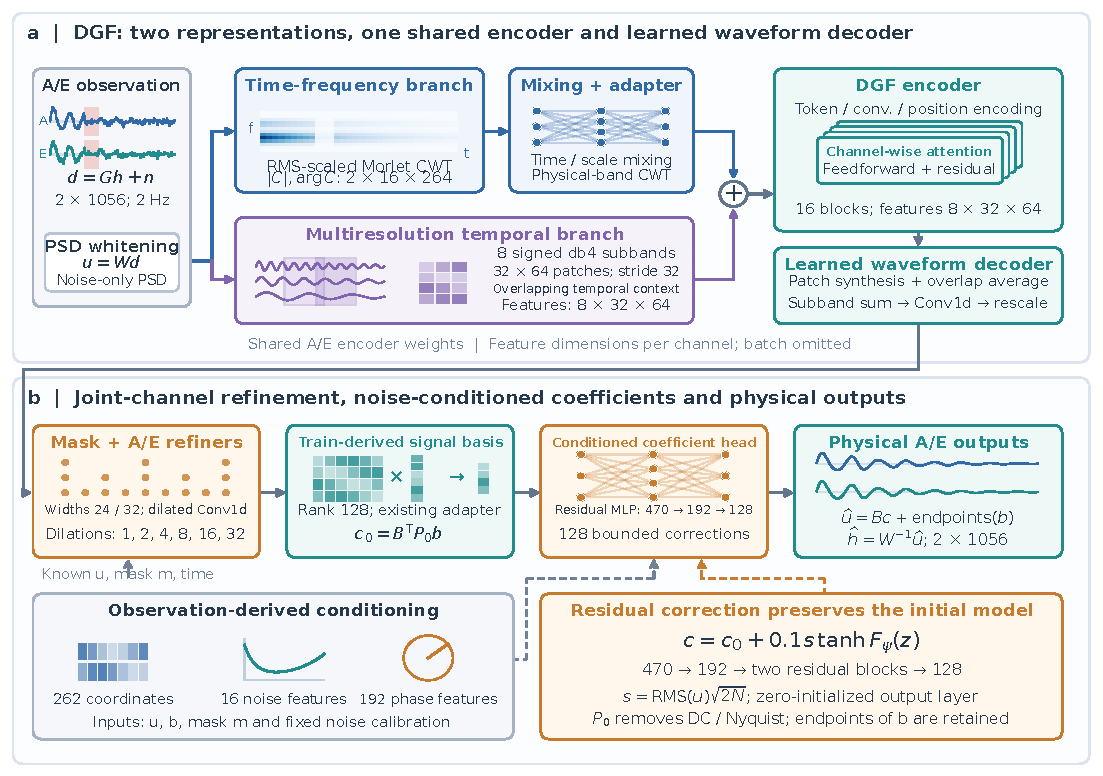
\includegraphics[width=\textwidth]{architecture_dgf_20261015.pdf}
\caption{Implemented DGF reconstruction architecture. (a) Fixed PSD whitening precedes the two shared-weight channel encoders. Blue and purple identify the oscillatory and temporal representations; green identifies fusion and waveform synthesis. (b) Mask-aware and joint $A/E$ refiners feed a training-derived signal-basis correction. The orange coefficient head receives observation-derived noise and continuous-phase features and returns a bounded coefficient residual. $P_0$ removes the DC and Nyquist components; the existing prediction's endpoint components are restored before inverse whitening. Solid arrows show the principal feature or waveform path, and dashed arrows identify conditioning inputs. Waveform, time-frequency, subband-patch and network icons are schematic. Encoder feature shapes are given per $A/E$ channel, with the batch dimension omitted.}\label{fig:pipeline}\label{fig:architecture}
\end{figure*}

\subsection{Joint-channel refinement and noise-conditioned coefficients}\label{sec:coefficients}
A channel-wise mask-aware residual module receives the observation, intermediate prediction, mask and normalized time coordinate. Its six dilated Conv1d blocks have width 24, kernel size 7 and dilations $1,2,4,8,16,32$, with group normalization and GELU. A second width-32 residual module couples the $A$ and $E$ predictions using the same dilation schedule.

A joint signal basis $B\in\mathbb R^{2N\times128}$ is fitted from the normalized, endpoint-excluded directions of the 60,000 clean training signals in whitened coordinates. Its columns are the leading eigenvectors of the training-direction second moment. The basis and original coefficient adapter give a whitened prediction $b$. They establish a compact signal representation, with each source contributing equally to basis construction.

The added residual head corrects the coefficients of $b$:
\begin{align}
c_0&=B^{\mathsf T}P_0b,\qquad
c=c_0+0.1s\tanh F_\psi(z),\label{eq:refinement}\\
\widehat u&=Bc+(I-P_0)b,\qquad
\widehat h=W^{-1}\widehat u.\nonumber
\end{align}
Here $P_0$ removes DC and Nyquist separately in each channel, and $s=\operatorname{RMS}(u)\sqrt{2N}$ with a numerical RMS floor. The existing prediction's endpoint components are retained. A zero-initialized final layer reproduces the starting coefficient prediction to floating-point precision.

The 470-dimensional input $z$ contains 262 normalized waveform, coefficient and mask coordinates; 16 absolute-noise and spectral-energy features; and 192 pooled continuous-phase features. The noise features use endpoint-excluded observed RMS, the independently calibrated noise RMS, coarse observed frequency-band energy ratios and RMS residuals between observation and prediction. For the physical-frequency CWT, continuous phase is encoded as
\begin{equation}
a_C\{1,\cos\theta_C,\sin\theta_C\},\quad
a_C=\log(1+|C|),\quad\theta_C=\arg C.\label{eq:continuous_phase}
\end{equation}
Amplitude weighting makes the phase features approach zero as the local CWT amplitude approaches zero. Pooling these features to a $4\times8$ grid in each channel gives 192 entries. The head maps 470 inputs to width 192, applies two residual MLP blocks and outputs 128 coefficients. Each residual block uses layer normalization, two linear layers, GELU and dropout 0.05. The additional head has 264,128 parameters. The complete stored model has 9,589,685 parameters.

All coefficient-head inputs are functions of the observation, existing prediction, known mask and fixed pure-noise calibration. The source parameters, true SNR and clean target supply simulation or supervision information during dataset construction and training.

\subsection{Direct mismatch, training objective and source separation}\label{loss}
We define the direct joint-channel inner product by
\begin{equation}
(a|b)_S=4\Delta f\operatorname{Re}
\sum_{c\in\{A,E\}}\sum_{k=1}^{N/2-1}
\frac{\widetilde a_{c,k}\widetilde b_{c,k}^{*}}{S_{c,\rm cal}(f_k)},\label{eq:joint_inner}
\end{equation}
where $\widetilde a=\Delta t\,\operatorname{rfft}(a)$, $\Delta t=1/f_s$ and $\Delta f=f_s/N$. The direct mismatch and full-window optimal signal norm are
\begin{equation}
\mathcal M_{AE}=1-\frac{(h|\widehat h)_S}{\sqrt{(h|h)_S(\widehat h|\widehat h)_S}},\quad
\rho^2=(h|h)_S.\label{eq:joint_mismatch}
\end{equation}
Each comparison uses the observation's fixed time and phase conventions. The signed normalized overlap gives $\mathcal M_{AE}\in[0,2]$, with values above one for anticorrelated predictions. A global positive rescaling of the PSD cancels between numerator and denominator. Frequency-dependent weighting determines the relative contribution of each bin.

The objective for the new coefficient and selective-fine-tuning stages is
\begin{equation}
\mathcal L=\mathcal M_{AE}+0.2E_S+0.02E_{\rm time,gap},\label{eq:loss}
\end{equation}
with
\begin{align}
E_S&=\frac{(\widehat h-h|\widehat h-h)_S}{(h|h)_S},\nonumber\\
E_{\rm time,gap}&=\frac{\sum_{c,j}(1+2m_j)(\widehat h_{c,j}-h_{c,j})^2}{\sum_{c,j}h_{c,j}^2}.\label{eq:auxiliary_errors}
\end{align}
These terms supervise both phase and amplitude on the full sequence and emphasize the masked interval in the physical-time residual. Source-level losses and population mismatches are averaged arithmetically with equal weights.

Figure~\ref{fig:training_workflow} separates data construction, optimization and independent testing. The complete training population contains 60,000 distinct physical sources. Three observations per source comprise two independently specified variable-width gaps and a third fixed 33-s gap with an additional independent physical-noise realization. Selected views also apply a global sign flip to both observation and target. All CWT and db4 features are recomputed from the corresponding observation. One full epoch therefore contains 180,000 views of 60,000 sources.

The validation population contains 1,500 disjoint sources. Its primary score is the full-population mean direct mismatch for uniformly sampled variable gap widths. Fixed 33- and 50-s masks are secondary diagnostics on those same validation sources. The predeclared final test contains 6,000 new source-disjoint seeds; its signals and observations are generated after model selection. Full-population results retain every generated source, with SNR-conditioned summaries reported alongside their explicit retained counts.

\begin{figure*}[t]
\centering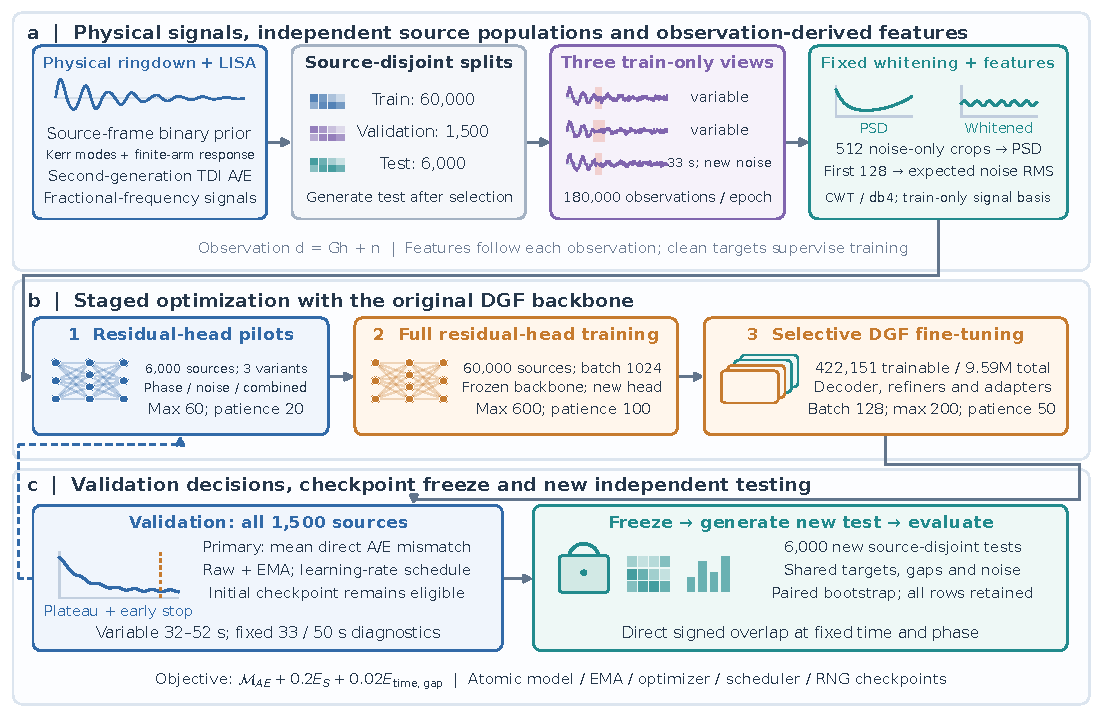
\includegraphics[width=\textwidth]{training_workflow_dgf_20261015.pdf}
\caption{Source-separated data and staged training workflow for the physical $A/E$ experiment. The three augmentation views use training sources only. The basis, PSD and expected noise RMS are fixed from clean training directions or independent pure-noise examples as indicated. Pilot stages compare the added head's conditioning blocks on identical training sources. The selected configuration is trained on the full source population, followed by selective decoder and adaptation-module fine-tuning. Validation governs candidate selection, learning-rate reduction and early stopping; model weights and protocol are frozen before the new independent test is generated. Solid arrows show the main workflow and the dashed return arrow denotes validation control of the optimization stages. Epoch limits are configured budgets. The waveform, PSD, optimization-curve and comparison icons are schematic; quantitative results are reported separately.}\label{fig:training_workflow}
\end{figure*}

\subsection{Staged optimization and reproducibility}\label{sec:training}
The saved DGF checkpoint and its physical-frequency and signal-basis adapters initialize the backbone. Three head-input configurations retain continuous phase with absolute-noise features set to zero, retain absolute-noise features with the added phase block set to zero, or retain both blocks. Each pilot uses the same 6,000 training sources, at most 60 epochs and patience 20 after a minimum of 20 epochs. The lowest complete validation-population mismatch selects the configuration; an exact tie selects the combined configuration. This is a conditioning-head comparison with a shared backbone.

The selected head configuration starts with a zero-initialized output layer and is trained on all 60,000 sources. Cached backbone predictions and observation features permit efficient training of the 264,128 added parameters. AdamW uses batch size 1024, weight decay $3\times10^{-4}$, a five-epoch warmup to learning rate $3\times10^{-4}$ and plateau-based reductions by a factor of two. The maximum budget is 600 epochs, with minimum 100, patience 100 and improvement threshold $10^{-6}$.

Selective fine-tuning updates the decoder, physical-frequency adapter, channel-wise and joint refiners, existing coefficient adapter and new head. This stage trains 422,151 parameters while preserving the encoder and fixed transforms. Group learning rates range from $5\times10^{-7}$ for the decoder to $10^{-4}$ for the new head. It uses batch size 128, the same weight decay, a 200-epoch maximum, minimum 40 and patience 50. The scheduler reduces learning rates after a validation plateau.

Raw and exponential-moving-average weights, with EMA factor 0.995, are compared using the same complete validation score. The initial checkpoint remains an eligible candidate. Every completed epoch atomically saves raw and EMA model states, optimizer and scheduler states, shuffle state and CPU/CUDA random states. Checkpoint selection uses the primary validation mean; fixed-gap and SNR-conditioned diagnostics accompany each candidate. Appendix~\ref{app:model_analysis} records the remaining numerical conventions.

\section{Retained legacy benchmark results}\label{sec:results}
The numerical statistics and result plots in this section are retained from the earlier phenomenological experiment. Its waveform, noise and training conventions are recorded in Appendix~\ref{app:sequence_modeling}; its noise units and single-channel construction define the scope of the following values. The new physical $A/E$ test follows Sec.~\ref{sec:method} and will replace these entries after the registered run completes.\par

In the earlier experiment we compare the original DGF checkpoint, the first refinement, and the selected augmented refinement on identical final-test observations and clean targets. The test seeds are 2026240000--2026240999, disjoint from the registered refinement training and validation ranges. All 1000 examples, including failures, contribute to the primary statistics. Linear interpolation replaces masked samples using neighboring noisy observations and leaves the observed samples unchanged. It measures gap bridging with the original noisy context, whereas DGF estimates the full clean waveform.

\subsection{Direct waveform mismatch}\label{subsec:Mismatch}
The time-domain normalized overlap and mismatch are
\begin{equation}
\mathcal M_t=1-\frac{\sum_jh_j\widehat h_j}{\sqrt{\sum_jh_j^2\sum_j\widehat h_j^2}}.
\end{equation}
For a noise-weighted comparison we define
\begin{align}
(a|b)_S&=4\Delta f\operatorname{Re}\sum_{k=1}^{T/2-1}\frac{\widetilde a_k\widetilde b_k^*}{S_{\rm cal}(f_k)},\\
\mathcal M_S&=1-\frac{(h|\widehat h)_S}{\sqrt{(h|h)_S(\widehat h|\widehat h)_S}},\label{eq:mismatch}
\end{align}
where $\widetilde a_k=\Delta t\,\mathrm{rFFT}(a)_k$, $T=1056$, $\Delta t=0.5$ s, and $\Delta f=1/(T\Delta t)$. The primary metric uses the rectangular segment and excludes DC and Nyquist. The shared normalization constants cancel in the overlap. Both metrics use the original time and phase conventions. With signed real overlaps, mismatch lies in $[0,2]$ and can exceed one for an anticorrelated reconstruction. A low PSD increases a frequency bin's relative contribution to the normalized inner product. A constant rescaling of the entire PSD leaves Eq.~\eqref{eq:mismatch} unchanged.

\begin{table*}[t]\centering
\caption{Direct reconstruction mismatch for all 1000 final-test examples. All waveforms contribute, with fixed time and phase conventions. Mean values are arithmetic means over examples. Interpolation acts on the noisy observed context and retains the original noise outside the mask.}\label{tab:results}
\begin{tabular}{lrrrr}\hline\hline
Predictor & Mean $\mathcal M_t$ & Mean $\mathcal M_S$ & Median $\mathcal M_S$ & 95th percentile $\mathcal M_S$\\\hline
Original DGF & 0.02537 & 0.02715 & 0.00444 & 0.09803 \\
First refinement & 0.00817 & 0.00863 & 0.00211 & 0.01534 \\
Augmented refinement & 0.00504 & 0.00537 & 0.00152 & 0.01014 \\
Linear interpolation & 0.13794 & 0.20933 & 0.07820 & 0.77879 \\
\hline\hline\end{tabular}\end{table*}

The augmented refinement reduces the population mean $\mathcal M_S$ by 80.2\% relative to the original DGF checkpoint and by 37.8\% relative to the first refinement. The paired mean differences are $-0.02178$ and $-0.003257$, with 95\% percentile bootstrap intervals $[-0.02697,-0.01696]$ and $[-0.00535,-0.00134]$, respectively. These intervals use a fixed bootstrap seed (20261009) and 5000 paired resamples of the test examples and quantify sampling variation for the fixed fitted checkpoints; training-seed variability requires replicated training runs. Figure~\ref{fig:mismatch} shows the complete empirical distributions. The mean, median, and upper percentiles characterize different aspects of the error tail and describe separate distributional properties.
\begin{figure*}[t]\centering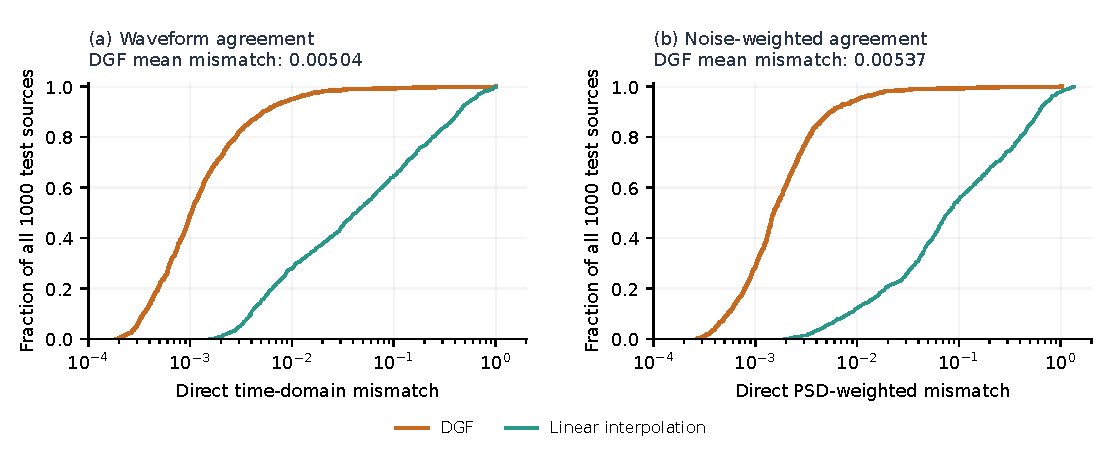
\includegraphics[width=\textwidth]{mismatch_cdf_presented.pdf}
\caption{Empirical distributions of direct time-domain and calibrated-noise-weighted mismatch for the same 1000 test examples. Each curve includes every example; the logarithmic horizontal axis resolves the low-mismatch region and the complete upper tail. The annotations compare the original and augmented population means. Interpolation retains noise outside the mask.}\label{fig:mismatch}\end{figure*}

\subsection{Gap location and successful reconstructions}
The clean-envelope peak lies inside the gap for 121 examples. In this subgroup the mean $\mathcal M_S$ is 0.14016 for original DGF, 0.04580 for the first refinement, and 0.02771 for the augmented refinement. The latter has median 0.00320 and 95th percentile 0.11283. The paired mean difference relative to the first refinement is $-0.01809$, with 95\% bootstrap interval $[-0.03427,-0.00172]$. For the remaining 879 examples, the augmented mean is 0.00229. Thus an improvement in the complete population coexists with substantially harder peak-masking cases.

Figure~\ref{fig:examples} illustrates high-fidelity recovery when the clean-envelope peak falls inside the gap. The panels show the three smallest augmented direct PSD mismatches among the 121 peak-masking sources: $4.08\times10^{-4}$, $4.89\times10^{-4}$ and $5.40\times10^{-4}$. Their suppressed intervals contain 28.6\%, 30.2\% and 29.9\% of the target's time-domain squared norm. These selected successful cases demonstrate recovery of informative masked signal content. The complete 1000-source population supplies Table~\ref{tab:results} and the distributional comparisons. Appendix~\ref{app:complementary} records central and difficult cases.
\begin{figure*}[t]\centering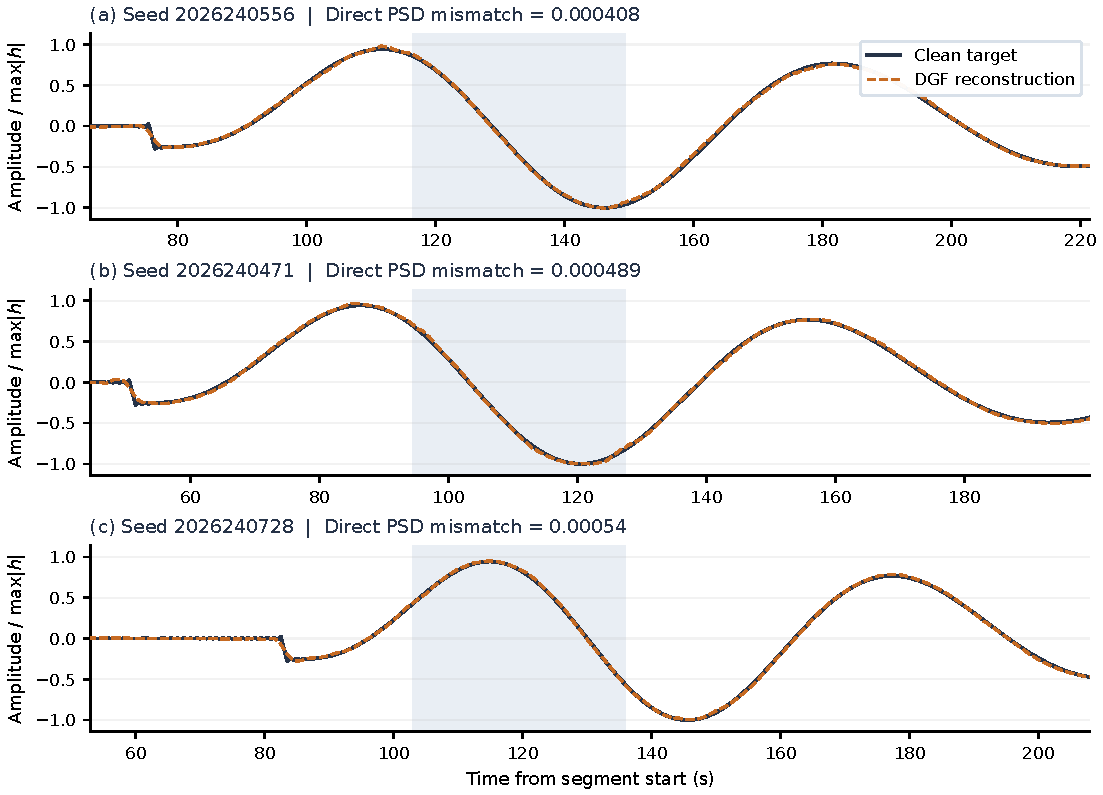
\includegraphics[width=\textwidth]{examples_best_peak.pdf}
\caption{High-fidelity reconstructions selected at ranks 1, 2 and 3 in ascending augmented direct PSD mismatch within the 121-source clean-envelope-peak-in-gap subgroup. Shading identifies each 33-s signal-suppression interval. Within each panel, the clean target and both stored predictions are divided by the same target peak amplitude for display; mismatches use the original arrays with fixed time and phase. The complete population contributes to Table~\ref{tab:results} and Fig.~\ref{fig:mismatch}.}\label{fig:examples}\end{figure*}

\subsection{Amplitude and spectral fidelity}\label{subsec:MeanSquaredError}\label{subsec:AmplitudeDensityFrequencySpectrum}
Normalized overlap is insensitive to an overall positive amplitude factor. We therefore also report $E=\|\widehat h-h\|_2/\|h\|_2$. Its augmented mean is 0.06496, median 0.04753, and 95th percentile 0.14741; the original DGF mean is 0.13370. The mean signed norm bias, $\|\widehat h\|_2/\|h\|_2-1$, is $-0.00200$, and its interpretation is complemented by absolute and relative residual diagnostics.

Inside the 121 peak-containing masks, $\|m(\widehat h-h)\|_2/\|mh\|_2$ has augmented mean 0.12349 and median 0.05735, compared with an original-model mean of 0.33401. The per-example archive retains local errors and their normalizations, alongside gap error normalized by the complete target norm. Appendix~\ref{app:complementary} records the sensitivity of this local measure to weak target content inside the gap.

Figure~\ref{fig:psd} compares the ensemble mean periodogram of the prediction error $\widehat h-h$ with that of the simulated noise. This measures frequency-dependent reconstruction error for the simulated family. Weak-component fidelity requires a component-resolved comparison.
\begin{figure}[tbp]\centering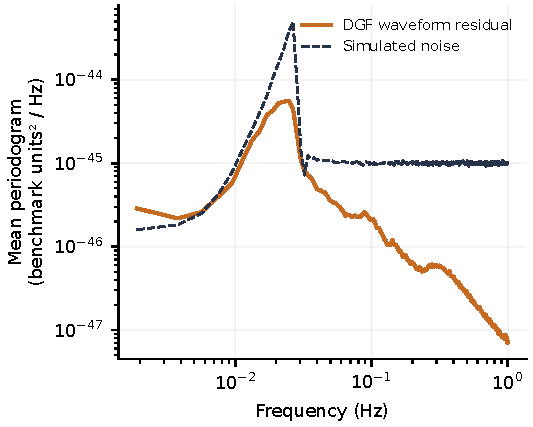
\includegraphics[width=\columnwidth]{error_psd_presented.pdf}
\caption{Mean one-sided periodograms of the simulated noise and of original/refined prediction errors over all 1000 test examples. Units are benchmark amplitude squared per hertz. The error spectrum characterizes reconstruction residuals in this earlier benchmark.}\label{fig:psd}\end{figure}

The independent Hann-window sensitivity check preserves the model ranking; Appendix~\ref{app:complementary} gives its weighting and numerical values.

\subsection{Phase recovery and alignment}\label{subsec:PhaseRecoveryAlignment}
Let $z=h+i\mathcal H[h]$ and $\widehat z=\widehat h+i\mathcal H[\widehat h]$. At the target-envelope peak $j_\star$, we define the wrapped phase diagnostic
\begin{equation}\Delta\phi_\star=\arg[\widehat z_{j_\star}z_{j_\star}^*],\qquad |\Delta\phi_\star|\in[0,\pi].\end{equation}
The phase diagnostic uses the unaligned prediction and fixed time convention. This measures the effective phase of the composite analytic waveform. The augmented mean absolute deviation is $1.50^\circ$, median $0.73^\circ$, 90th percentile $2.69^\circ$, and 95th percentile $4.08^\circ$. The original-model mean is $4.32^\circ$. Figure~\ref{fig:phase} pairs the complete phase-error distribution with the successful peak-masking waveform from Fig.~\ref{fig:examples}(b). Its peak-phase error is $0.096^\circ$. Appendix~\ref{app:complementary} gives the peak-masking subgroup statistics and the dependence on observed signal strength.
\begin{figure*}[t]\centering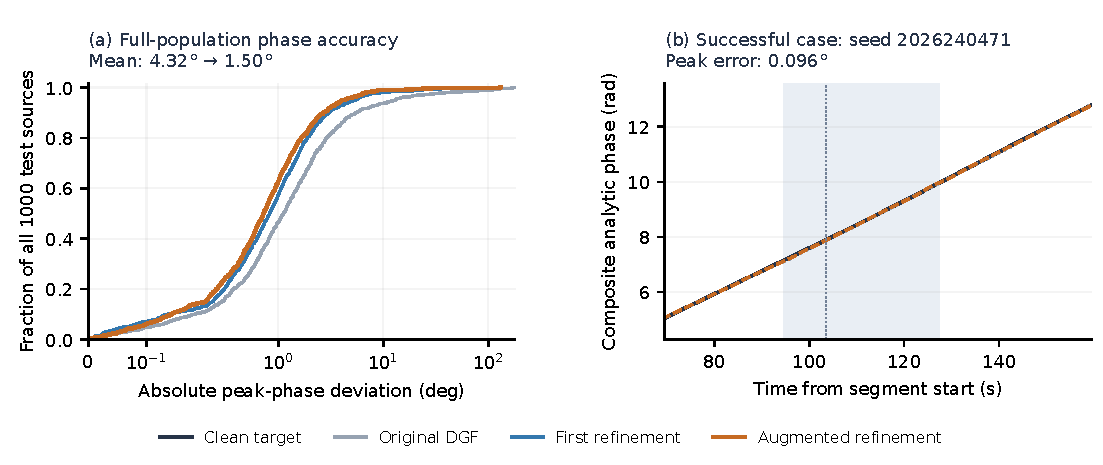
\includegraphics[width=\textwidth]{phase_presented.pdf}
\caption{(a) Complete absolute peak-phase distributions for all 1000 sources, with a linear central region and logarithmic scale above $0.2^\circ$. (b) Composite analytic phase for seed 2026240471, the successful waveform in Fig.~\ref{fig:examples}(b). The clean and predicted phases use a common unwrapped branch; their relative phase modulo $2\pi$ is preserved. Phase curves are displayed where the clean analytic-envelope amplitude exceeds 10\% of its peak. Shading marks the signal-suppression interval, and the vertical dotted line identifies the target-envelope peak. The predictions retain the original time and phase convention.}\label{fig:phase}\end{figure*}

\subsection{Refinement ablation}
A separate matched-budget experiment compares refinement using a time-domain objective alone, adding the explicit mask, adding spectral terms, and adding both. It uses 2048 unique training waveforms with two masks each, the same 1500 validation examples, three initialization seeds per variant, and at most 100 epochs with patience 20. The composite validation scores, averaged over the three seeds, are 0.03004, 0.02657, 0.02719, and 0.02440, respectively; the mask-plus-spectrum variant performs best in each seed. This supports the refinement design under the stated small-budget protocol. Its scope is the refinement module under this small-budget protocol. Controlled retraining of the original branches and replication of the long run require additional experiments. Variant selection uses validation data.

\section{Discussion and Conclusions}\label{sec:discussion}
DGF combines complex time--frequency information with signed multiresolution temporal context to estimate a clean ringdown waveform from noisy, partially suppressed signal observations. The physical $A/E$ extension preserves the original encoder--decoder and introduces fixed PSD whitening, explicit gap and joint-channel refiners, a train-derived signal basis and observation-derived noise conditioning. These modules define a consistent path from simulated fractional-frequency observations to reconstructed fractional-frequency outputs.

The present methods specify a finite 528-s analysis window, approximately 6\%--10\% variable signal-suppression intervals, a nonspinning progenitor prior and an idealized equal-arm LISA/TDI response with stationary instrument noise. The earlier numerical benchmark remains a separately labeled reference during revision. The new full-population direct mismatch, paired model comparisons, amplitude residuals and SNR-conditioned counts will provide the quantitative assessment of this extension after independent testing.

The scientific motivation is preservation of the ringdown's oscillatory structure for subsequent analysis. The direct signed overlap uses the observation's fixed time and phase convention, while relative waveform and spectral residuals assess amplitude fidelity. Error distributions and explicit difficult-case diagnostics describe the accuracy across the specified population. Individual-mode frequency, phase and damping-time recovery requires dedicated component-resolved validation.

Extension to a moving unequal-arm response, nonstationary instrument noise, confusion foregrounds, overlapping sources and multiple intervals requires simulations and comparisons under those conditions. The deterministic reconstruction supplies a point estimate conditioned on the observed data. Calibrated conditional uncertainty and replicated training runs would quantify additional uncertainty in waveform recovery and model fitting.

For downstream parameter inference, the observation likelihood should use the original residual $d-Gh(\theta)$ and the appropriate noise covariance. Reconstructed samples are correlated functions of the original observation. DGF can supply initial waveforms or sampling proposals, with posterior accuracy and coverage assessed against that observation likelihood. The calculation of detection evidence and tests of black hole spectroscopy therefore requires a separate inference study.

Related reconstruction and data-augmentation methods~\cite{Baghi2019,Blelly2021,Xu_2024,Mao:2025cae,Wang:2024waveformer} motivate shared-benchmark comparisons. Such comparisons should fix the source population, response, noise, gap definition, train/test separation and overlap convention. The workflow developed here makes these choices explicit and retains the original DGF reconstruction task as the basis for that evaluation.
\begin{acknowledgments}
The authors thank He Wang and Yiyang Guo for helpful discussions. This research is supported in part by the National Key R\&D Program of China, grant number 2020YFC2201300, and the National Natural Science Foundation of China, grant numbers 12035016, 12375058 and 12361141825.



\end{acknowledgments}
\appendix
\section{Implementation and reproducibility}\label{app:model_analysis}
\subsection{Representations and active sequence operation}
For one $A/E$ channel, the legacy CWT array is $2\times16\times264$, and the subband patches and branch outputs are $8\times32\times64$. Fusion is elementwise addition. For a channel's feature matrix $Z\in\mathbb R^{32\times64}$, the active attention operation is
\begin{equation}
A(Z)=\operatorname{softmax}(ZZ^{\mathsf T}/\sqrt{64})Z.
\end{equation}
Each of the eight feature channels uses this operation, followed by learned feedforward transformations, residual connections and normalization. The legacy class also stores allocated multihead-attention parameters; the active forward operation is the expression above. Stored parameter totals consequently describe the checkpoint representation. Sequence context spans the full window.

The db4 implementation selects its approximation and seven detail components from the library coefficient ordering. Learned decoded channels are combined by overlap averaging and subband summation. The decoder's linear patch map has checkpoint values independent of the encoder embedding map. The loading procedure clones the initial transposed storage before reading the two checkpoint tensors, preserving their stored values on CPU and GPU.

\subsection{Numerical and test conventions}
The white-space RMS floor is $10^{-4}$ for coefficient and residual normalization. Training spectral target and prediction squared norms are floored at $10^{-12}$ for finite numerical division, and physical-time relative-error denominators use the same floor in the scaled working representation. Physical evaluation uses float64 transforms, the common frozen PSD and the complete target norm. Overlap is clipped to $[-1,1]$ to bound roundoff. A zero prediction is assigned mismatch one; a zero target triggers a dataset validation failure.

The registered final physical test uses 6,000 source seeds 2038200000--2038205999. The new fixed-gap training-noise stream uses 2158200000--2158259999; all corresponding transforms are recomputed from the generated observations. Raw and EMA checkpoints, full training histories, independent noise calibration, masks, seeds and per-source predictions define the reproducibility archive. Source and fixed-asset SHA-256 manifests are checked throughout the run. Training restoration uses the last fully completed epoch, preserving optimizer, scheduler and random states.

The source prior and injected response peak define event-centered simulation windows and mask metadata. Inference inputs consist of the resulting observation, known mask and fixed preprocessing arrays. Clean target arrays enter training losses and evaluation diagnostics. The reconstruction code is available at \url{https://github.com/ljq2088/RingdownGapFilling}; the archived configurations and selected-checkpoint identifiers accompany the final evaluation.

\section{Earlier benchmark and retained numerical results}\label{app:sequence_modeling}
This appendix identifies the data and training prescription associated with the numerical values retained in Sec.~\ref{sec:results}. The preceding physical $A/E$ methods define the revised experiment.
\subsection{Earlier signal prescription}
The earlier generator contains four oscillatory components with the legacy labels $(2,2)$, $(2,1)$, $(3,3)$, and $(4,4)$. The generator draws independent uniform coordinates $M\in[10^5,10^6]$, $q\in[0.5,0.8]$, and $z\in[4,6]$, with fixed orientation and phase conventions. The mass coordinate enters the generator through $M T_\odot$, and $z$ sets a distance scale. These are the numerical waveform-family coordinates used by that experiment. The revised mass convention is specified in Sec.~\ref{sec:physical_signals}.

Writing $\eta=q/(1+q)^2$ and $\chi=\eta(2\sqrt{3}-3.5171\eta+2.5763\eta^2)$, the implemented frequencies and decay times are
\begin{align}
\omega_a^{\rm b}&=\frac{f_{1a}+f_{2a}(b_a-\chi)^{f_{3a}}}{M T_\odot},\label{eq:benchmark_frequency}\\
\tau_a^{\rm b}&=\frac{2[q_{1a}+q_{2a}(1-\chi)^{q_{3a}}]}{\omega_a^{\rm b}},
\end{align}
with $b_a=(1,1,3,4)$ in the component order above. Table~\ref{tab:frequency_coefficients} records the coefficients. The standard Kerr fits use $b_a=1$ for every mode~\cite{berti2006gravitational}; the third and fourth components use the altered $b_a$ values recorded here. The labels identify the components of this earlier numerical family.
\begin{table}[t]
\caption{Coefficient values retained by the benchmark. The factors $b_a$ in Eq.~\eqref{eq:benchmark_frequency} differ from the standard Kerr prescription for the last two rows.}\label{tab:frequency_coefficients}
\centering\begin{tabular}{crrrrrr}\hline\hline
Label & $f_1$ & $f_2$ & $f_3$ & $q_1$ & $q_2$ & $q_3$\\\hline
$22$ &1.5251&-1.1568&0.1292&0.7000&1.4187&-0.4990\\
$21$ &0.6000&-0.2339&0.4175&-0.3000&2.3561&-0.2277\\
$33$ &1.8956&-1.3043&0.1818&0.9000&2.3430&-0.4810\\
$44$ &2.3000&-1.5056&0.2244&1.1929&3.1191&-0.4825\\\hline\hline
\end{tabular}\end{table}
The implemented component multipliers are
\begin{align}
A_{22}^{\rm b}&=0.303+0.571\eta,& A_{21}^{\rm b}&=0.060+0.099\eta,\nonumber\\
A_{33}^{\rm b}&=0.671+0.157\eta,& A_{44}^{\rm b}&=0.122-0.188\eta-0.964\eta^2.
\end{align}
They are numerical coefficients of this benchmark. They retain the numerical coefficients of the original experiment, with the $21$ and $33$ ordering shown explicitly. The physical excitation prescription of Sec.~\ref{sec:physical_signals} uses the relative-amplitude fits of Ref.~\cite{Kamaretsos2012}. Fixed angular factors and a TianQin-inspired modulation are applied in frequency space, followed by a discrete inverse transform, a cyclic shift, a 1056-sample crop, and an amplitude factor of 0.03. This earlier response is the frequency-space modulation specified below.

\subsection{Signal discretization}
The frequency-domain function \texttt{sf} is evaluated on \texttt{arange}$(10^{-5},1,10^{-5})$ Hz, containing $K=99999$ entries. The response-modulated sum of its four components is treated as the input to \texttt{irfft} with $N=2(K-1)=199996$, using the library's $1/N$ inverse normalization. The first entry at $10^{-5}$ Hz is assigned the DC position by this operation, and no continuous-Fourier-to-DFT sampling-rate factor is applied. The series is cyclically shifted by $N/2$ samples and cropped from $(N-1056)/2+s$ with a random integer $s\in[0,527]$. The crop is cast to float32 and multiplied by 0.03. This procedure specifies the retained benchmark; its discrete normalization defines the numerical waveform arrays used for the earlier comparison.

Fixed angles are $\iota=\pi/4$, $\gamma=\pi/3$, $\theta_d=1.17662$, $\psi_d=-0.873302$, and $\phi_d=-0.615727$ radians, with the legacy TianQin-inspired modulation frequency approximately $1.99\times10^{-5}$ Hz. These fixed angular and modulation choices specify the earlier response. The remnant and detector conventions for the revised population are given in Sec.~\ref{sec:physical_signals}.

\subsection{Noise discretization and evaluation weighting}
Let $u_j$ be independent standard Gaussian variates on the parent sequence and let $S_{\rm ref}$ denote the Welch spectrum of the supplied channel combination. The implementation first interpolates this PSD onto the generator grid, then interpolates its square root onto the parent real-FFT grid. Denoting the resulting array by $B_k$, the synthesized sequence is
\begin{equation}n_j^{\rm parent}=\sqrt{f_s}\,\operatorname{irfft}\left[\frac{\operatorname{rfft}(u)_k}{\sqrt N}B_k\right]_j,\qquad f_s=2\,\mathrm{Hz}.
\end{equation}
It is cropped centrally to 1056 samples and cast to float32. Away from endpoint bins, the normalization gives an ensemble one-sided PSD $2B_k^2/N$ before cropping. Window leakage in a short crop further changes the frequency-dependent spectrum. $S_{\rm cal}$ is therefore estimated from independently reserved cropped noise examples on the actual evaluation grid. The Hann sensitivity check uses a periodic Hann window and the correspondingly calibrated windowed-noise PSD.

The empirical PSD includes the synthetic process and its out-of-band fill. Inverse-PSD weighting emphasizes the corresponding low-noise bins. Population statistics average each source mismatch equally and retain the complete generated population.

\subsection{Earlier noise and refinement stages}
The earlier reference spectrum was estimated from a supplied three-series file after the combination $n_A=(n_Z-n_X)/\sqrt{2}$, using Welch segments of length 1024 and a 15-s sampling interval. The file supplied numerical arrays; detector-generation, unit and full-provenance metadata were unavailable. Frequencies outside its reference range were filled with $10^{-40}$ in numerical PSD units. A separate calibration of 200 cropped noise examples supplied the evaluation spectrum for Sec.~\ref{sec:results}.

The earlier refinement used 12,000 training waveforms, 1,500 validation sources, and then six train-only noise/mask views per source. Its objective weighted the mask-enhanced relative time error, relative complex spectral error and direct spectral mismatch by $1$, $1/2$ and $1/4$. A composite validation score weighted the full population and the peak-containing subgroup by $0.75$ and $0.25$. The augmented run selected epoch 1095 within its 1200-epoch limit. Its 1,000 final-test seeds were 2026240000--2026240999. These conventions specify the retained historical results and training curve.
\begin{figure}[tbp]\centering\includegraphics[width=\columnwidth]{training.pdf}
\caption{Retained validation history from the earlier numerical benchmark. The population mismatch and composite score use the historical weighting described in this appendix. This plot records the earlier run; Fig.~\ref{fig:training_workflow} specifies the revised physical $A/E$ training protocol.}\label{fig:loss}\end{figure}


\section{Complementary benchmark diagnostics}\label{app:complementary}
This appendix documents the earlier benchmark's distributional limits and sensitivity checks alongside the successful reconstructions displayed in the main text. Every numerical population statistic uses the same complete set of 1000 test sources.
\subsection{Central and difficult waveform cases}
Figure~\ref{fig:complementary_examples} retains examples selected at the median, 90th percentile and maximum augmented direct PSD mismatch. The maximum mismatch is 1.01221 and the maximum absolute peak-phase deviation is $130.09^\circ$; these sources contribute to the population statistics. In the maximum-mismatch case, seed 2026240571, the 126--159-s gap contains the clean-envelope peak and 92.85\% of the target's time-domain squared norm. Its augmented prediction has 46.24\% of the target norm. The earlier refinement's mismatch for this source is 0.48104, recording case-level variation across fitted predictors. Reconstruction uncertainty requires a conditional uncertainty model in addition to a point estimate.
\begin{figure*}[t]\centering\includegraphics[width=\textwidth]{examples.pdf}
\caption{Complementary earlier-benchmark cases selected at ranks 500, 900 and 1000 after sorting the augmented direct PSD mismatch across all 1000 sources. The clean target and stored original/augmented outputs use fixed time and phase and the generator's numerical amplitude units. Gray shading identifies the 33-s signal mask.}\label{fig:complementary_examples}\end{figure*}
\subsection{Phase tails, amplitude ratio and local normalization}
For the 121 sources with clean-envelope peaks inside the gap, the augmented mean absolute peak-phase deviation is $5.20^\circ$ and the 95th percentile is $19.93^\circ$. Figure~\ref{fig:complementary_phase} gives the full phase distributions and mismatch versus the numerical amplitude ratio $R=\|h\|_2/\|n\|_2$.
\begin{figure*}[t]\centering\includegraphics[width=\textwidth]{phase_and_R.pdf}
\caption{Complementary population diagnostics for every earlier-benchmark source. Left: absolute target-peak composite Hilbert-phase deviations. Right: direct PSD mismatch versus the unweighted numerical waveform-to-noise norm ratio $R$. All 1000 points per predictor are retained.}\label{fig:complementary_phase}\end{figure*}
The gap-local relative error $\|m(\widehat h-h)\|_2/\|mh\|_2$ becomes ill conditioned when the clean target is almost zero inside a late gap. Its full-population mean is 12.12, reflecting this local normalization. Gap errors normalized by the complete target norm accompany these local diagnostics in the evaluation archive.
\subsection{Window sensitivity}
A periodic Hann window is applied to both waveforms and paired with an independently calibrated noise PSD using that same window. Mean direct mismatches are 0.04736, 0.01647 and 0.01116 for original DGF, first refinement and augmented refinement. These values preserve the ranking under the stated window convention. Windowing changes the relative emphasis on parts of the finite segment; the primary comparison uses the declared rectangular-window weighting.

\bibliography{DGF_references}
\end{document}
